\section{Elevation dataset description and Visualisation}


\subsection{Distribution and Topographical Profile}

The distribution of all valid elevation values was analyzed to understand the region's topographical profile.

\begin{figure}[H]
    \centering
    % Placeholder for the Elevation Histogram
    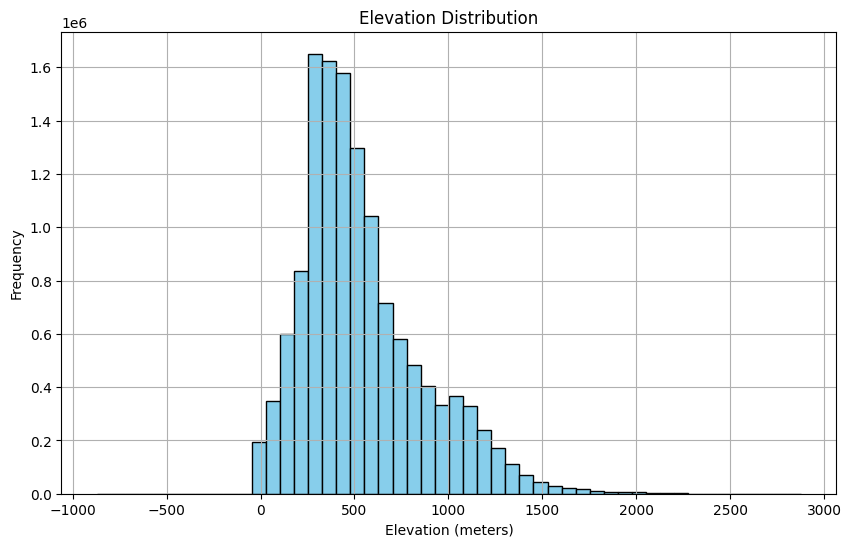
\includegraphics[width=0.5\textwidth]{images/Elevation/Elevation Distribution.png}
    \caption{Frequency distribution of elevation values in the merged Elevation Dataset. The distribution exhibits a clear left skew.}%
    \label{fig:elevation_histogram}
\end{figure}

\textbf{Histogram Interpretation}
The elevation histogram exhibits a \textbf{left-skewed distribution}. This indicates that low-elevation areas dominate the region, while higher elevations occur less frequently, forming a long left tail. The majority of the terrain is therefore concentrated in low to mid-elevation ranges, corresponding to coastal plains and steppe regions, with higher elevations associated with inland mountain ranges.
\begin{figure}[H]
    \centering
    % Placeholder for the Elevation Boxplot
    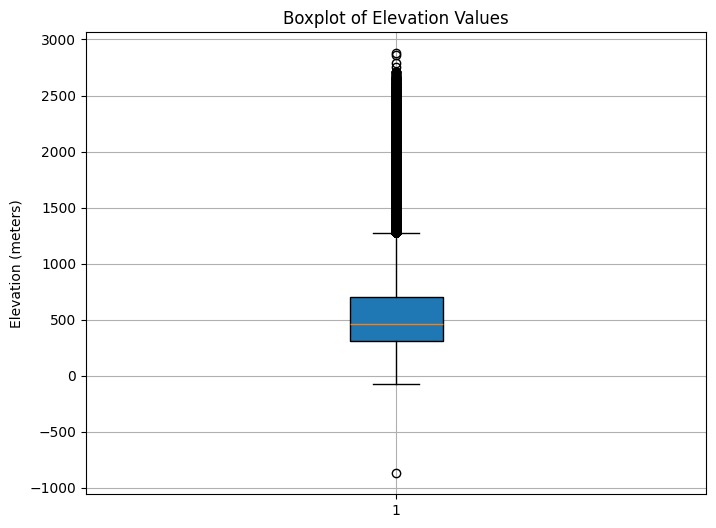
\includegraphics[width=0.5\textwidth]{images/Elevation/elevation box plot.png}
    \caption{Boxplot summarizing the elevation data, highlighting the interquartile range (IQR) and the presence of extreme high-elevation outliers.}%
    \label{fig:elevation_boxplot}
\end{figure}

\textbf{Boxplot Interpretation}
The boxplot confirms the presence of significant high-elevation \textbf{outliers}. These extreme values correspond to the highest points in the study area, notably the \textbf{Tassili n’Ajjer} and the \textbf{Hoggar Mountains (Ahaggar)} in southern Algeria, which reach peak elevations of approximately 2100 to 3000 meters.

